\chapter{Release 1: Speed and Angle Estimation}
\label{chap:speed-angle}

\section{Introduction}
This chapter presents the technical background and implementation work for speed and angle estimation within the EYES video analytics solution. The work described here corresponds to Sprint 1 of the project, which focused on developing the foundational components for measuring object speed and heading direction from video streams.

Accurate estimation of object speed and heading direction is essential for a variety of surveillance and safety applications, including traffic monitoring, anomaly detection, and predictive analysis. The speed and angle estimation module operates as part of the broader EYES pipeline, receiving tracking information from upstream detection and tracking modules.

Sprint 1 aimed to establish the core infrastructure for speed and angle estimation, including the state of the art study, mathematical foundations, pipeline architecture, and initial implementation with configuration parameters.

\section{Sprint 1 Development}

\subsection{Sprint Backlog For Sprint 1}

The Sprint 1 backlog focused on building the foundational components for speed and angle estimation. The main tasks included:

\begin{itemize}
  \item Research and document state-of-the-art methods for speed estimation
  \item Research and document state-of-the-art methods for angle and heading estimation
  \item Design and implement the speed estimation pipeline architecture
  \item Develop mathematical foundations for speed, curvature, and angle calculations
  \item Implement EMA smoothing for temporal filtering
  \item Address implementation challenges including sparse trajectories and calibration dependency
  \item Define and document configuration parameters for pipeline tuning
\end{itemize}

\subsubsection{Resources and Datasets}

\paragraph{Models Used}
\begin{itemize}
  \item \textbf{YOLOv8n} [3]: Nano version of YOLOv8 for object detection (6.3MB)
  \item \textbf{YOLOv8s}: Small version for better accuracy (22MB)
  \item Pre-trained on COCO dataset (80 classes)
\end{itemize}

\paragraph{Datasets}
\begin{itemize}
  \item \textbf{COCO Dataset} [4]: Common Objects in Context, used for pre-training
  \item \textbf{Internal Dataset}: Collected using EYES data collector (confidential under NDA)
\end{itemize}

\paragraph{Libraries and Frameworks}
\begin{center}
\renewcommand{\arraystretch}{1.2}
\begin{tabular}{|p{0.25\textwidth}|p{0.20\textwidth}|p{0.45\textwidth}|}
\hline
\textbf{Library} & \textbf{Version} & \textbf{Purpose} \\
\hline
PyTorch & 2.0+ & Deep learning framework \\
\hline
Ultralytics & 8.0+ & YOLOv8 implementation \\
\hline
OpenCV & 4.8+ & Image processing, video handling \\
\hline
NumPy & 1.24+ & Numerical computations \\
\hline
\end{tabular}
\captionof{table}{Libraries and frameworks used}
\label{tab:libraries}
\end{center}

\subsection{State of the Art Study}

\subsubsection{Speed Estimation Methods}

\paragraph{Pixel-Based Methods}
Pixel-based speed estimation operates directly in the image coordinate space without explicit geometric transformation. Given the centroid position $(x_t, y_t)$ at frame $t$, the pixel displacement is computed as:

\begin{equation}
\Delta p = \sqrt{(x_{t+1} - x_t)^2 + (y_{t+1} - y_t)^2}
\end{equation}

The speed in pixels per frame is then:

\begin{equation}
v_{pixel} = \frac{\Delta p}{\Delta t}
\end{equation}

where $\Delta t = 1/fps$ is the time between consecutive frames. While computationally simple, pixel-based methods suffer from perspective distortion, as the relationship between pixel displacement and real-world distance varies with the object's position in the image. Objects farther from the camera appear smaller and move fewer pixels per unit of real-world distance compared to objects closer to the camera.

\paragraph{Homography-Based Methods}
\label{subsec:homography}

Homography-based approaches address the perspective distortion problem by transforming image coordinates to a top-down view of the scene. A homography matrix $\mathbf{H}$ maps points from the image plane to a world coordinate system:

\begin{equation}
\begin{bmatrix} x_w \\ y_w \\ w \end{bmatrix} = \mathbf{H} \begin{bmatrix} x_i \\ y_i \\ 1 \end{bmatrix}
\end{equation}

where $(x_i, y_i)$ are image coordinates and the world coordinates are obtained as $(X, Y) = (x_w/w, y_w/w)$. The full homography matrix is:

\begin{equation}
\mathbf{H} = \begin{bmatrix} h_{11} & h_{12} & h_{13} \\ h_{21} & h_{22} & h_{23} \\ h_{31} & h_{32} & h_{33} \end{bmatrix}
\end{equation}

\begin{figure}[h]
\centering
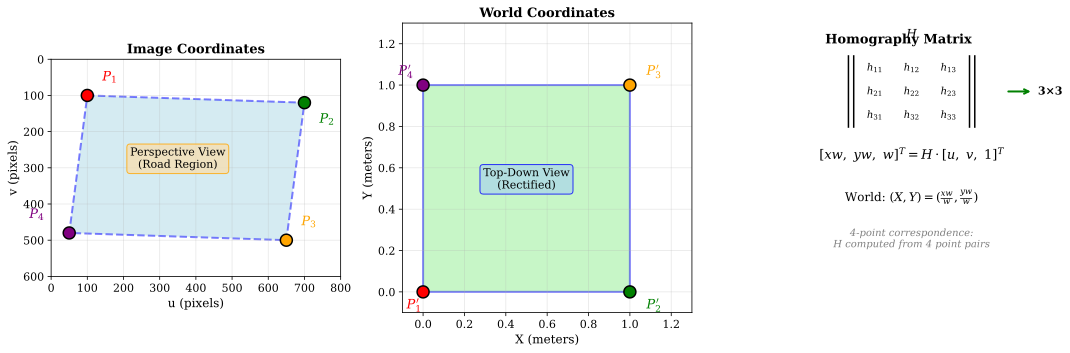
\includegraphics[width=\textwidth]{images/homography_transform.png}
\caption{Homography transformation from image coordinates to world coordinates [5] - Simplified diagram showing four point correspondences used to compute the $3 \times 3$ homography matrix for jury understanding.}
\label{fig:homography}
\end{figure}

The homography matrix is typically estimated from at least 4 point correspondences using the Direct Linear Transform (DLT) algorithm with RANSAC for robustness against outliers. Once calibrated, the homography enables accurate distance and speed measurements in real-world units.

The primary advantage of homography-based methods is their ability to provide physically meaningful measurements. However, they require accurate calibration and assume a planar ground surface, which may not hold in all deployment scenarios.

\paragraph{Optical Flow Methods}
Optical flow estimates the apparent motion of pixels between consecutive frames by analyzing intensity patterns. The optical flow field $\mathbf{u}(x, y)$ at each pixel provides a dense representation of motion:

\begin{equation}
I(x, y, t) = I(x + u_x, y + u_y, t + \Delta t)
\end{equation}

where $I$ is the image intensity and $(u_x, u_y)$ is the flow vector. Methods such as the Lucas-Kanade algorithm or Horn-Schunck approach compute flow by assuming brightness constancy and spatial coherence:

\begin{equation}
I_x u + I_y v + I_t = 0
\end{equation}

where $I_x, I_y$ are spatial image gradients and $I_t$ is the temporal gradient. For speed estimation, optical flow can be aggregated over object regions to estimate the average motion magnitude.

While optical flow provides rich motion information, it is sensitive to illumination changes, occlusions, and aperture problems. Additionally, converting optical flow to physical speed still requires knowledge of the camera geometry and scene scale.

\paragraph{Deep Learning-Based Methods}
Recent advances in deep learning have enabled end-to-end speed estimation from video frames. Convolutional neural networks (CNNs) and recurrent architectures can learn to predict speed directly from spatiotemporal features without explicit geometric modeling. 3D CNN architectures capture spatio-temporal features from sequences of consecutive frames, while hybrid approaches combine optical flow computation with CNN processing for speed regression.

Deep learning methods offer the potential to handle complex scenarios and implicit scene understanding. However, they introduce additional computational overhead and require substantial training data, which may not be practical for all deployment contexts. Furthermore, the black-box nature of neural networks can complicate error analysis and calibration.

\subsubsection{Angle and Heading Estimation Methods}

\paragraph{Trajectory-Based Methods}
Trajectory-based heading estimation computes the direction of motion from the object's trajectory over time. Given a sequence of positions $\{(x_1, y_1), (x_2, y_2), \ldots, (x_n, y_n)\}$, the heading angle $\theta$ can be estimated using the four-quadrant inverse tangent:

\begin{equation}
\theta = \arctan2(\Delta y, \Delta x)
\end{equation}

where $\Delta x$ and $\Delta y$ represent the displacement between trajectory points. In world coordinates (after homography transformation), this becomes:

\begin{equation}
\theta_t = \arctan2(y_{w,t+1} - y_{w,t}, x_{w,t+1} - x_{w,t})
\end{equation}

The choice of points for computing displacement affects the estimation quality: using immediate neighbors provides responsiveness but is sensitive to noise, while using points further apart improves stability but reduces responsiveness to rapid directional changes.

\paragraph{Curvature-Based Methods}
For objects following curved paths, the instantaneous heading can be derived from the local curvature of the trajectory. The curvature $\kappa$ at a point is defined as:

\begin{equation}
\kappa = \frac{|\mathbf{v} \times \mathbf{a}|}{|\mathbf{v}|^3}
\end{equation}

where $\mathbf{v}$ is the velocity vector and $\mathbf{a}$ is the acceleration vector. In component form:

\begin{equation}
\kappa = \frac{|x'y'' - y'x''|}{(x'^2 + y'^2)^{3/2}}
\end{equation}

\begin{figure}[h]
\centering
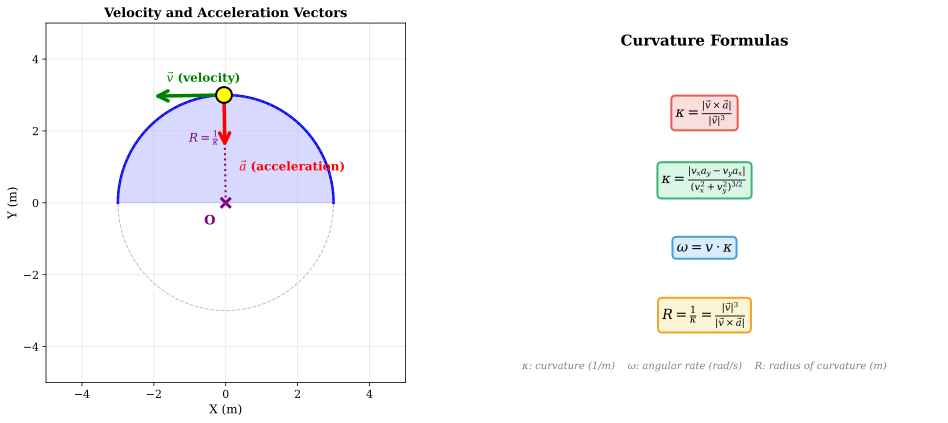
\includegraphics[width=\textwidth]{images/curvature_calculation.png}
\caption{Curvature calculation from trajectory points showing velocity and acceleration vectors - Simplified diagram for jury understanding.}
\label{fig:curvature}
\end{figure}

The angular rate of change $\omega$ is then computed from the curvature and speed:

\begin{equation}
\omega = v \cdot \kappa
\end{equation}

Curvature-based methods provide smooth heading estimates that naturally account for turning behavior. However, they require higher-order derivatives of position, which can amplify noise in the trajectory data.

\paragraph{Angular Rate Integration}
An alternative approach estimates the angular rate directly from trajectory changes. The angular rate can be computed from consecutive velocity vectors:

\begin{equation}
\omega = \frac{d\theta}{dt} = \frac{v_x a_y - v_y a_x}{v_x^2 + v_y^2}
\end{equation}

where $(v_x, v_y)$ and $(a_x, a_y)$ are the velocity and acceleration components. This formulation provides a direct estimate of the turning rate without explicit curvature computation.

\subsubsection{Workflow Comparison}

This section provides a comparative analysis of the four main approaches to speed estimation, examining their pipelines, advantages, limitations, and practical considerations.

\paragraph{Pixel-Based Workflow}
The pixel-based workflow represents the simplest approach to speed estimation, operating entirely in image coordinates without geometric transformation.

\textbf{Pipeline}: Video → Detection → Centroid Tracking → Pixel Displacement → Speed

The pixel-based method computes speed directly from centroid displacement between frames. While computationally efficient, this approach suffers from fundamental limitations:

\begin{itemize}
  \item \textbf{No perspective correction}: Objects at different distances from the camera have different pixel-to-world scale factors
  \item \textbf{Scale varies with distance}: The same real-world speed produces different pixel displacements depending on object position
  \item \textbf{No physical units}: Speed is reported in pixels per frame, which lacks physical meaning
\end{itemize}

\textbf{Use case}: Quick prototyping, non-critical applications where absolute accuracy is not required.

\paragraph{Homography-Based Workflow (Our Implementation)}
The homography-based workflow addresses the fundamental limitation of pixel-based methods by transforming image coordinates to a world coordinate system.

\textbf{Pipeline}: Video → Detection → Tracking → Homography Transform → World Coordinates → Speed + Angle

This approach offers several advantages over simpler methods:

\begin{itemize}
  \item \textbf{Perspective corrected}: The homography transformation accounts for the geometric relationship between the image plane and the ground plane
  \item \textbf{Real-world units}: Speed is computed in meters per second, providing physically meaningful measurements
  \item \textbf{Angle estimation}: Heading direction can be computed accurately in world coordinates
  \item \textbf{Deterministic}: The transformation is mathematically well-defined and debuggable
\end{itemize}

\textbf{Requirements}: 4-point calibration, planar ground assumption. The calibration process requires marking four known points in the image and specifying their real-world coordinates.

\paragraph{Optical Flow Workflow}
Optical flow methods estimate motion by analyzing the apparent movement of brightness patterns between consecutive frames.

\textbf{Pipeline}: Video → Feature Detection → Optical Flow → Motion Vectors → Aggregation → Speed

Advantages of the optical flow approach include:

\begin{itemize}
  \item \textbf{Dense motion field}: Motion is estimated at every pixel, providing rich spatial information
  \item \textbf{No explicit tracking needed}: The flow field captures motion without requiring object detection and tracking
  \item \textbf{Sub-pixel accuracy}: Modern optical flow algorithms can estimate motion with sub-pixel precision
\end{itemize}

However, optical flow methods face several challenges:

\begin{itemize}
  \item \textbf{Illumination sensitive}: Changes in lighting can produce spurious flow vectors
  \item \textbf{Aperture problem}: Local flow estimation is inherently ambiguous in homogeneous regions
  \item \textbf{Calibration still required}: Converting flow to physical speed requires knowledge of scene geometry
\end{itemize}

\paragraph{Deep Learning Workflow}
Deep learning approaches leverage neural networks to learn speed estimation directly from video data.

\textbf{Pipeline}: Video Sequence → 3D CNN/Transformer → Speed Regression

The deep learning workflow offers unique advantages:

\begin{itemize}
  \item \textbf{Learned features}: The network automatically discovers relevant features for speed estimation
  \item \textbf{Handles complex scenarios}: Can potentially handle non-planar surfaces, occlusions, and unusual camera configurations
  \item \textbf{End-to-end optimization}: The entire pipeline can be optimized jointly for the target task
\end{itemize}

Challenges with deep learning methods include:

\begin{itemize}
  \item \textbf{Training data required}: Large labeled datasets with ground truth speeds are necessary
  \item \textbf{Computational overhead}: Neural network inference requires significant computational resources
  \item \textbf{Black-box nature}: Difficult to debug and understand failure modes
  \item \textbf{Domain adaptation}: Models trained on one scene may not generalize to different camera configurations
\end{itemize}

\begin{center}
\renewcommand{\arraystretch}{1.2}
\begin{tabular}{|p{0.20\textwidth}|p{0.15\textwidth}|p{0.18\textwidth}|p{0.18\textwidth}|p{0.15\textwidth}|}
\hline
\textbf{Approach} & \textbf{Accuracy} & \textbf{Computational Cost} & \textbf{Calibration} & \textbf{Real-time} \\
\hline
Pixel-based & Low & Low & None & Yes \\
\hline
Homography (ours) & High & Medium & 4-point & Yes \\
\hline
Optical Flow & Medium & Medium & Required & Marginal \\
\hline
Deep Learning & High & High & Learned & Hardware-dependent \\
\hline
\end{tabular}
\captionof{table}{Comparison of speed estimation workflows}
\label{tab:workflow-comparison}
\end{center}

\begin{figure}[h]
\centering
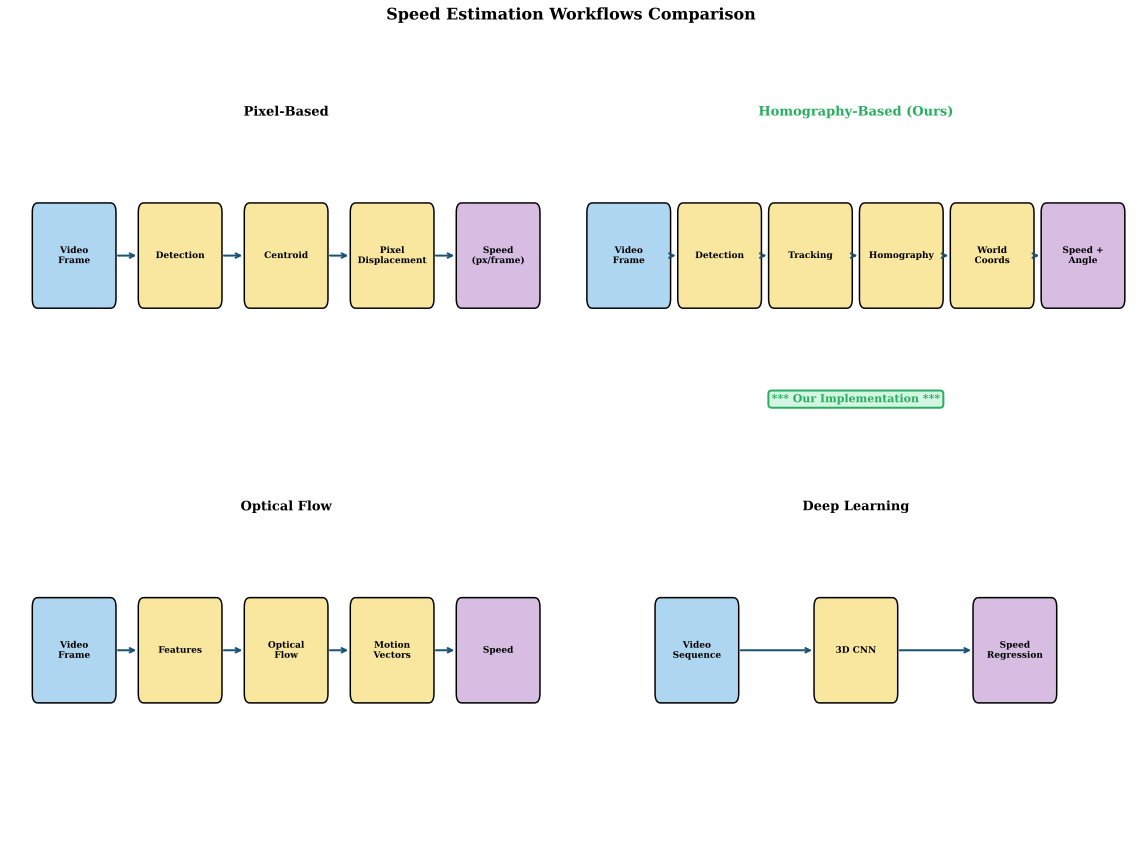
\includegraphics[width=\textwidth]{images/workflow_comparison.png}
\caption{Comparison of speed estimation workflows showing the data flow and components of each approach - Simplified diagram for jury understanding.}
\label{fig:workflow-comparison}
\end{figure}

\subsubsection{Comparison with Existing Solutions}

This section compares our implementation with existing speed estimation solutions in the literature and industry.

\paragraph{Ultralytics YOLO Speed Estimation [1]}
The Ultralytics YOLO framework provides a built-in speed estimation module that uses a simplified approach for converting pixel measurements to real-world units:

\begin{itemize}
  \item \textbf{Scale conversion}: Uses a \texttt{meter\_per\_pixel} parameter for linear pixel-to-meter conversion
  \item \textbf{No perspective correction}: Simple linear scaling without homography matrix transformation
  \item \textbf{Limited output}: Provides speed estimation only, with no angle or heading information
  \item \textbf{Tracking method}: Uses centroid tracking for position estimation
\end{itemize}

This approach is suitable for scenarios with minimal perspective distortion but lacks the geometric accuracy provided by homography-based methods.

\paragraph{OpenCV-based Approaches [2]}
Traditional OpenCV-based speed estimation implementations typically employ straightforward distance calculations:

\begin{itemize}
  \item \textbf{Distance formulas}: Often use simple Euclidean distance between detected object centroids
  \item \textbf{Manual calibration}: Require manual specification of scale factors without automatic perspective correction
  \item \textbf{Limited scope}: Focus primarily on speed estimation without angle or heading capabilities
  \item \textbf{No smoothing}: Generally lack temporal filtering for noise reduction
\end{itemize}

These approaches prioritize simplicity over accuracy and do not address the full range of motion analysis requirements.

\paragraph{Our Implementation Advantages}
The implemented solution offers several advantages over existing approaches:

\begin{itemize}
  \item \textbf{Full homography transformation}: Proper perspective correction using a $3 \times 3$ homography matrix calibrated from four point correspondences [5]
  \item \textbf{Dual estimation}: Provides both speed AND angle/heading estimation in world coordinates
  \item \textbf{Curvature-based analysis}: Implements turning metrics including curvature and angular rate computation
  \item \textbf{EMA smoothing}: Applies exponential moving average filtering to reduce measurement noise
  \item \textbf{Physical constraints}: Enforces realistic acceleration and turn rate limits to reject implausible estimates
\end{itemize}

\subsection{Design Diagrams For Sprint 1}

\subsubsection{Pipeline Architecture}

The speed estimation pipeline was developed as part of Sprint 1 to provide real-time speed and angle measurements for detected objects. The architecture follows a modular design with well-defined interfaces between components.

\paragraph{Pipeline Modules}
The implementation consists of the following core modules:

\begin{center}
\renewcommand{\arraystretch}{1.2}
\begin{tabular}{|p{0.22\textwidth}|p{0.12\textwidth}|p{0.56\textwidth}|}
\hline
\textbf{Module} & \textbf{Lines} & \textbf{Responsibility} \\
\hline
\texttt{math.py} & 1045 & Speed estimation, turning metrics, trajectory analysis \\
\hline
\texttt{pipeline.py} & 2251 & End-to-end processing, RTSP handling, event clipping \\
\hline
\texttt{calibration.py} & 177 & Homography-based coordinate transformation \\
\hline
\texttt{detection.py} & 128 & YOLOv8 object detection wrapper \\
\hline
\end{tabular}
\captionof{table}{Core modules of the speed estimation pipeline}
\label{tab:modules}
\end{center}

\begin{figure}[h]
\centering
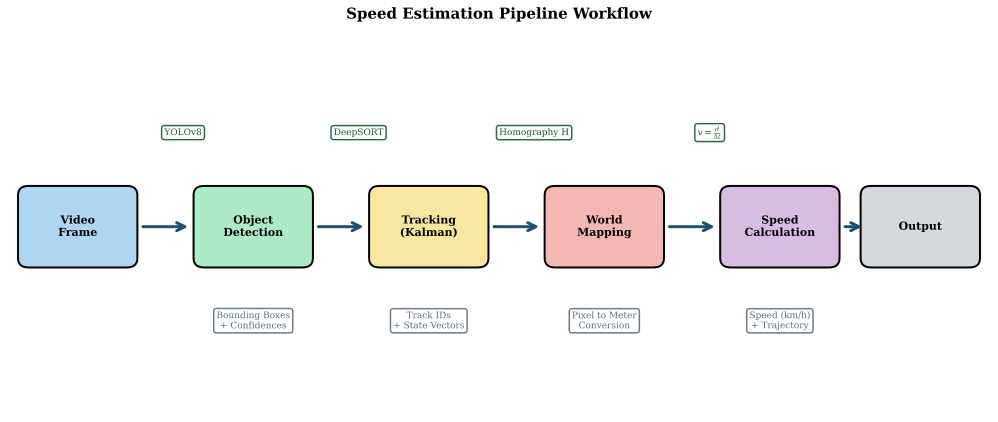
\includegraphics[width=\textwidth]{images/speed_estimation_workflow.png}
\caption{Speed estimation pipeline workflow showing data flow from video frames to speed output - Simplified diagram for jury understanding.}
\label{fig:workflow}
\end{figure}

\paragraph{Data Flow}
The processing pipeline follows these stages:

\begin{enumerate}
  \item \textbf{Detection}: YOLOv8 processes each video frame to produce bounding boxes with class labels and confidence scores.
  \item \textbf{Tracking}: An IoU-based tracker assigns persistent IDs to detections across frames.
  \item \textbf{World Mapping}: The bottom-center point of each bounding box is transformed from pixel to world coordinates using the homography matrix.
  \item \textbf{Trajectory Accumulation}: World coordinates are accumulated as trajectory dots with timestamps.
  \item \textbf{Speed Calculation}: Speed is computed from displacement between trajectory dots.
  \item \textbf{Turning Metrics}: Curvature and angular rate are computed from trajectory derivatives.
  \item \textbf{Smoothing Filter}: EMA smoothing is applied to produce stable estimates.
  \item \textbf{Constraint Validation}: Physical constraints are enforced and implausible estimates are flagged.
\end{enumerate}

\paragraph{Trajectory Dot System}
A key feature of the implemented pipeline is the trajectory dot system, which provides visual feedback for debugging and monitoring. The system maintains a buffer of recent trajectory points for each tracked object and renders them as a trail of dots on the display output.

\begin{figure}[h]
\centering
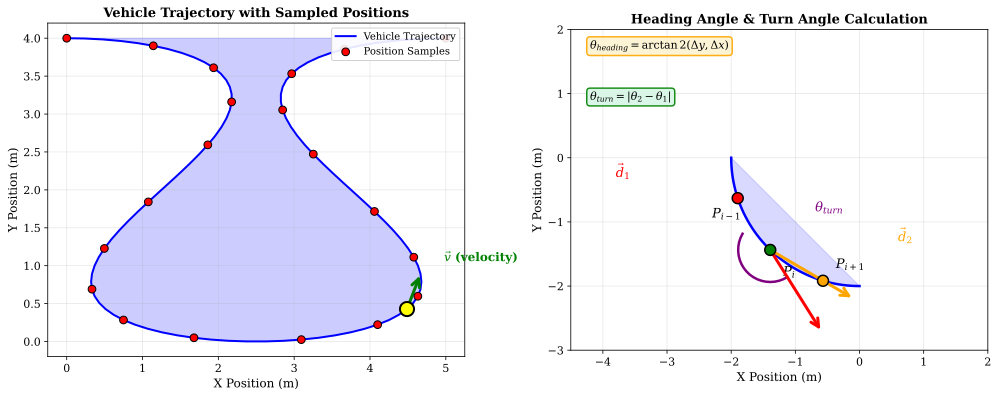
\includegraphics[width=\textwidth]{images/trajectory_analysis.png}
\caption{Trajectory analysis with dot visualization system showing motion history - Simplified diagram for jury understanding.}
\label{fig:trajectory}
\end{figure}

The system uses a trajectory dot approach where dots are added to each track's history when specific conditions are met:

\begin{equation}
\text{Add dot if: } |\Delta \mathbf{p}| \geq d_{min} \text{ and } \Delta t \geq t_{min}
\end{equation}

Default parameters are $d_{min} = 0.20$ meters and $t_{min} = 0.2$ seconds. This approach provides temporal smoothing by requiring minimum displacement before recording new trajectory points.

The trajectory dot system serves multiple purposes:
\begin{itemize}
  \item Visual verification of tracking continuity
  \item Assessment of trajectory smoothness and noise characteristics
  \item Debugging support for speed and angle estimation issues
  \item Presentation of motion history to operators
\end{itemize}

\subsubsection{Diagram Legend}

To facilitate understanding of the diagrams presented in this chapter, the following legend explains the visual elements used:

\paragraph{Visual Elements}
\begin{itemize}
  \item \textbf{Dots}: Represent trajectory points in world coordinates. Each dot corresponds to a recorded position of a tracked object at a specific timestamp.
  \item \textbf{Arrows}: Represent velocity vectors. The arrow direction indicates the heading of the object, and the length is proportional to the speed.
  \item \textbf{Curved lines}: Represent curvature calculation paths. These show the local trajectory segment used for computing curvature and angular rate.
  \item \textbf{Angles}: Computed using the $\arctan2$ formula, which provides the four-quadrant inverse tangent to determine heading direction from displacement components.
\end{itemize}

\paragraph{Coordinate Systems}
All diagrams use a right-handed coordinate system where:
\begin{itemize}
  \item The $X$-axis points to the right in the world frame
  \item The $Y$-axis points upward (or forward in the top-down view)
  \item Angles are measured counter-clockwise from the positive $X$-axis
\end{itemize}

\subsubsection{Mathematical Foundations}

\paragraph{Speed Calculation}
The fundamental speed calculation converts displacement between trajectory points into physical speed. Given two consecutive trajectory points in world coordinates $(x_1, y_1)$ and $(x_2, y_2)$ with timestamps $t_1$ and $t_2$, the speed $v$ is computed as:

\begin{equation}
v = \frac{\Delta d}{\Delta t} = \frac{\sqrt{(x_2 - x_1)^2 + (y_2 - y_1)^2}}{t_2 - t_1}
\end{equation}

The displacement $\Delta d$ is computed in world units (typically meters), yielding speed in physical units (meters per second). The homography transformation ensures that perspective effects are properly accounted for in the distance computation.

\paragraph{Curvature Computation}
For heading estimation, the pipeline computes the local curvature of the trajectory. Given three consecutive points $\mathbf{p}_1$, $\mathbf{p}_2$, and $\mathbf{p}_3$, the velocity and acceleration vectors at $\mathbf{p}_2$ are approximated as:

\begin{equation}
\mathbf{v} = \frac{\mathbf{p}_3 - \mathbf{p}_1}{2\Delta t}
\end{equation}

\begin{equation}
\mathbf{a} = \frac{\mathbf{p}_3 - 2\mathbf{p}_2 + \mathbf{p}_1}{\Delta t^2}
\end{equation}

The curvature $\kappa$ is then:

\begin{equation}
\kappa = \frac{|\mathbf{v} \times \mathbf{a}|}{|\mathbf{v}|^3}
\end{equation}

The angular rate $\omega$ represents the rate of change of the heading angle:

\begin{equation}
\omega = v \cdot \kappa = \frac{|\mathbf{v} \times \mathbf{a}|}{|\mathbf{v}|^2}
\end{equation}

\paragraph{EMA Smoothing}
Exponential Moving Average (EMA) smoothing is applied to reduce noise in speed and angle estimates. The EMA filter provides a simple yet effective temporal smoothing mechanism:

\begin{equation}
S_t = \alpha \cdot X_t + (1 - \alpha) \cdot S_{t-1}
\end{equation}

where $S_t$ is the smoothed value at time $t$, $X_t$ is the raw input value, and $\alpha \in (0, 1)$ is the smoothing factor. Lower values of $\alpha$ provide stronger smoothing but introduce more lag, while higher values preserve responsiveness but allow more noise to pass through.

\begin{figure}[h]
\centering
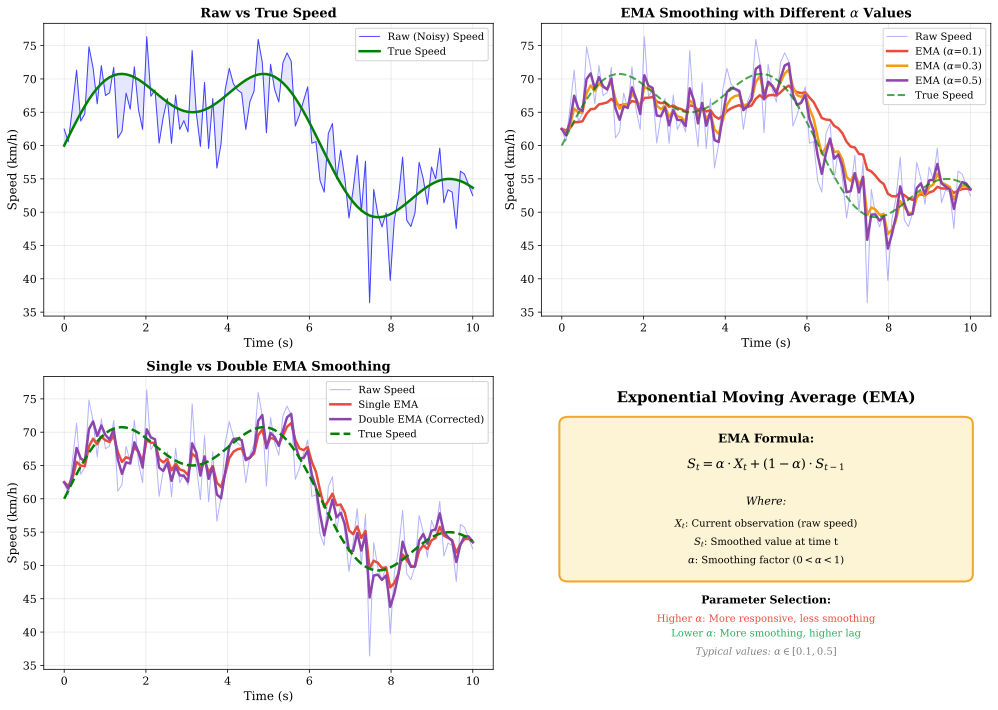
\includegraphics[width=\textwidth]{images/speed_smoothing.png}
\caption{Effect of EMA smoothing on speed estimates comparing raw and filtered values - Simplified diagram for jury understanding.}
\label{fig:smoothing}
\end{figure}

For angle estimation, special handling is required due to the circular nature of angles. The EMA filter is applied to the sine and cosine components separately:

\begin{equation}
\sin(S_t) = \alpha \cdot \sin(X_t) + (1 - \alpha) \cdot \sin(S_{t-1})
\end{equation}

\begin{equation}
\cos(S_t) = \alpha \cdot \cos(X_t) + (1 - \alpha) \cdot \cos(S_{t-1})
\end{equation}

The smoothed angle is then computed as:

\begin{equation}
S_t = \arctan2(\sin(S_t), \cos(S_t))
\end{equation}

\paragraph{Physical Constraints}
Physical constraints are enforced to reject implausible estimates and maintain consistency with real-world behavior:

\begin{itemize}
  \item \textbf{Maximum speed}: Estimates exceeding a configurable maximum speed threshold are flagged as invalid.
  \item \textbf{Minimum displacement}: Very small displacements are treated as zero velocity to avoid noise amplification.
  \item \textbf{Acceleration limits}: Changes in speed exceeding physical acceleration limits trigger smoothing or invalidation.
  \item \textbf{Angular rate limits}: Heading changes are bounded by plausible turning rates for the object class.
\end{itemize}

\subsection{Implementation Of Sprint 1}

\subsubsection{Implementation Challenges and Issues}

During Sprint 1, several implementation challenges were encountered and addressed. This section documents the key issues and their mitigations.

\paragraph{Sparse Trajectory Dots}
In scenarios with low frame rates or fast-moving objects, trajectory points may be sparse, leading to inaccurate speed and angle estimates. Sparse dots result in larger time intervals $\Delta t$, which amplifies the effect of positional noise.

\textbf{Mitigation}: The pipeline implements adaptive interpolation for sparse trajectories and applies stronger smoothing when the inter-frame interval exceeds a threshold. Additionally, a minimum number of trajectory points is required before producing estimates.

\paragraph{Zero Velocity False Positives}
Stationary objects or objects with minimal motion may produce spurious velocity estimates due to detection jitter. Small positional variations from the detection module can be misinterpreted as motion, leading to non-zero speed estimates for stationary objects.

\textbf{Mitigation}: A minimum displacement threshold is applied. Displacements below this threshold are classified as zero velocity. The threshold is configurable and can be tuned based on detection noise characteristics.

\paragraph{Heading Uncertainty at Low Speeds}
At low speeds, the trajectory direction becomes increasingly unreliable due to the dominance of positional noise over actual motion. This leads to erratic heading estimates for slow-moving or nearly stationary objects.

\textbf{Mitigation}: The heading estimation module implements a confidence measure based on speed magnitude. Below a minimum speed threshold, heading estimates are either withheld or marked as low confidence. The smoothed heading is maintained from the last reliable estimate.

\paragraph{Calibration Dependency}
The homography-based approach depends critically on accurate camera calibration. Errors in the homography matrix propagate to speed and angle estimates, potentially introducing systematic biases. Furthermore, calibration must be performed for each camera viewpoint, adding to deployment overhead.

\textbf{Mitigation}: The pipeline includes calibration validation checks that detect gross calibration errors by verifying expected geometric properties. Documentation for the calibration process was developed to ensure consistent setup across deployments.

\subsubsection{Configuration Parameters}

The speed and angle estimation pipeline exposes several configuration parameters that control its behavior. Table~\ref{tab:config-params} summarizes the key parameters and their default values.

\begin{center}
\renewcommand{\arraystretch}{1.2}
\begin{tabular}{|p{0.28\textwidth}|p{0.12\textwidth}|p{0.52\textwidth}|}
\hline
\textbf{Parameter} & \textbf{Default} & \textbf{Description} \\
\hline
\texttt{smoothing\_alpha} & 0.3 & EMA smoothing factor for speed estimates. Lower values provide stronger smoothing. \\
\hline
\texttt{angle\_smoothing\_alpha} & 0.2 & EMA smoothing factor for angle estimates. Applied to sine and cosine components separately. \\
\hline
\texttt{max\_speed\_mps} & 50.0 & Maximum valid speed in meters per second. Estimates exceeding this threshold are flagged. \\
\hline
\texttt{min\_displacement\_m} & 0.1 & Minimum displacement in meters for non-zero velocity detection. \\
\hline
\texttt{min\_speed\_for\_heading} & 0.5 & Minimum speed in m/s required for reliable heading estimation. \\
\hline
\texttt{trajectory\_buffer\_size} & 30 & Number of trajectory points retained for visualization and smoothing. \\
\hline
\texttt{max\_acceleration} & 10.0 & Maximum acceleration in m/s$^2$ for physical constraint validation. \\
\hline
\texttt{max\_angular\_rate} & 2.0 & Maximum angular rate in rad/s for heading change validation. \\
\hline
\texttt{min\_trajectory\_points} & 3 & Minimum trajectory points required before producing estimates. \\
\hline
\end{tabular}
\captionof{table}{Configuration parameters for speed and angle estimation}
\label{tab:config-params}
\end{center}

\subsection{References}
\begin{enumerate}
  \item Ultralytics, "Speed Estimation with YOLO", https://docs.ultralytics.com/fr/guides/speed-estimation/
  \item OpenCV Documentation, "Motion Analysis and Object Tracking"
  \item Ultralytics, "YOLOv8 Models", https://docs.ultralytics.com/models/yolov8/
  \item COCO Dataset, https://cocodataset.org/
  \item Zhang et al., "2D Homography for Traffic Data Collection", arXiv:2401.07220
\end{enumerate}

\section{Conclusion}
This chapter presented the work accomplished during Sprint 1, focusing on speed and angle estimation for tracked objects within the EYES video analytics framework. The implemented pipeline combines homography-based coordinate transformation, trajectory-based speed computation, curvature-derived heading estimation, and EMA smoothing to produce robust and physically meaningful estimates.

The state of the art review highlighted the trade-offs between different approaches, with homography-based methods offering the best balance of accuracy and practicality for fixed-camera deployments. The mathematical foundations established the core equations governing speed calculation, curvature computation, and temporal smoothing.

Several implementation challenges were encountered, including sparse trajectory dots, zero velocity false positives, heading uncertainty at low speeds, and calibration dependency. Mitigations were implemented and documented to address these issues.

The configuration parameters table provides a reference for tuning the pipeline to specific deployment requirements. The next chapter will extend this work to address additional estimation tasks and pipeline enhancements developed in subsequent sprints.
